\chapter{Implementation}\label{ch:methodology}
Mirroring the previously presented approach (Chapter~\ref{ch:approach}), we will describe the methodology used to develop the system.
The chapter is divided into four sections.
The first section will describe the data collection process, the second section will describe the data augmentation, the third section will describe the classification model, the fourth section will describe the virtual environment.

All these sections are included and merged in a single pipeline with a user friendly interface that connects the data augmentation or collection from the headset, classification model, and virtual environment.
The framework is plug-and-play, meaning that it can be easily extended to support new data augmentation or generation methods, classification models, virtual environments or real devices.
The framework is also designed to be easy to use, providing an easy user interface and only requiring the paths to the model files and the WebSocket address to send messages.


\section{Data Collection}
The data collection process is a crucial step in the development of a machine learning system.
It is used to gather the data necessary to train the machine learning model and is divided into two steps: the data collection and the data preprocessing.
The data collection step is used to gather the data necessary to train the machine learning model.
The data preprocessing step is used to clean the data and prepare it for training.
For the first step, we used publicly available EEG motor imagery datasets, such as the BCI Competition IV dataset 2a~\cite{tangermann2012review}, the Weibo~\cite{yi2014evaluation} and the PhysioNet EEG Motor Movement/Imagery Dataset~\cite{goldberger2000physiobank, schalk2004bci2000}.
These datasets contain EEG recordings of subjects performing motor imagery tasks, such as imagining moving their left or right hand, or their feet.
The datasets contains the preprocessed EEG recordings of the subjects, as well as the corresponding labels indicating the class to which the data point belongs.
It is important to notice that we perform some ulterior preprocessing steps, such as filtering and windowing, to clean, split and prepare the data for the training phase.
Also, due to the nature of the dataset recordings, the label distribution is highly unbalanced towards the resting state, so we decided to balance the dataset by undersampling all the data points to the same amount of samples, which was decided to be the lowest class count.
\subsection*{Parameters Used}
To obtain the data, we used the python library MOABB, wich, via the Motor Imagery paradigm, provides simplified access the datasets.
The Motor Imagery paradigm, via its constructor, allows to specify the preprocessing steps.
% In this project, we used the following parameters:
% \begin{itemize}
%     \item \textbf{Channels}: The channels used to record the EEG signals. In this project, we used the 58 channels presented in Figure~\ref{fig:eeg_channels}.
%     \item \textbf{Events}: The events used to label the data points. In this project, we used the left and right hand, feet and rest motor imagery events.
%     \item \textbf{Number of Output Classes}: The number of classes to which the data points belong. In this project, we used 4 classes.
%     \item \textbf{Cutoff Frequency for the Bandpass Filter}: The cutoff frequency used to filter the EEG signals. In this project, we used a cutoff frequency of 0.5\textemdash40 Hz.
%     \item \textbf{Epoch Start Time}: The time at which the epoch starts. In this project, we used a start time of 0 seconds.
%     \item \textbf{Epoch End Time}: The time at which the epoch ends. In this project, we used an end time of 0.5
%     \item \textbf{Resampling Frequency}: The frequency at which the data points are resampled. In this project, we used a resampling frequency of 128 Hz.
% \end{itemize}
% change bullet list to paragraph
Among the provided parameters, we provided the 58 channels used to record the EEG signals presented in Figure~\ref{fig:eeg_channels}, the ``left hand'', ``right hand'', ``feet'' and ``rest'' event labels to select the data points, 4 as the number of output classes, between 0.5 and 40 Hz as the cutoff frequency for the bandpass filter, the epoch start and end time, respectively 0 and 0.5 seconds, and the resampling frequency of 128 Hz.


\begin{figure}[!htbp]
    \centering
    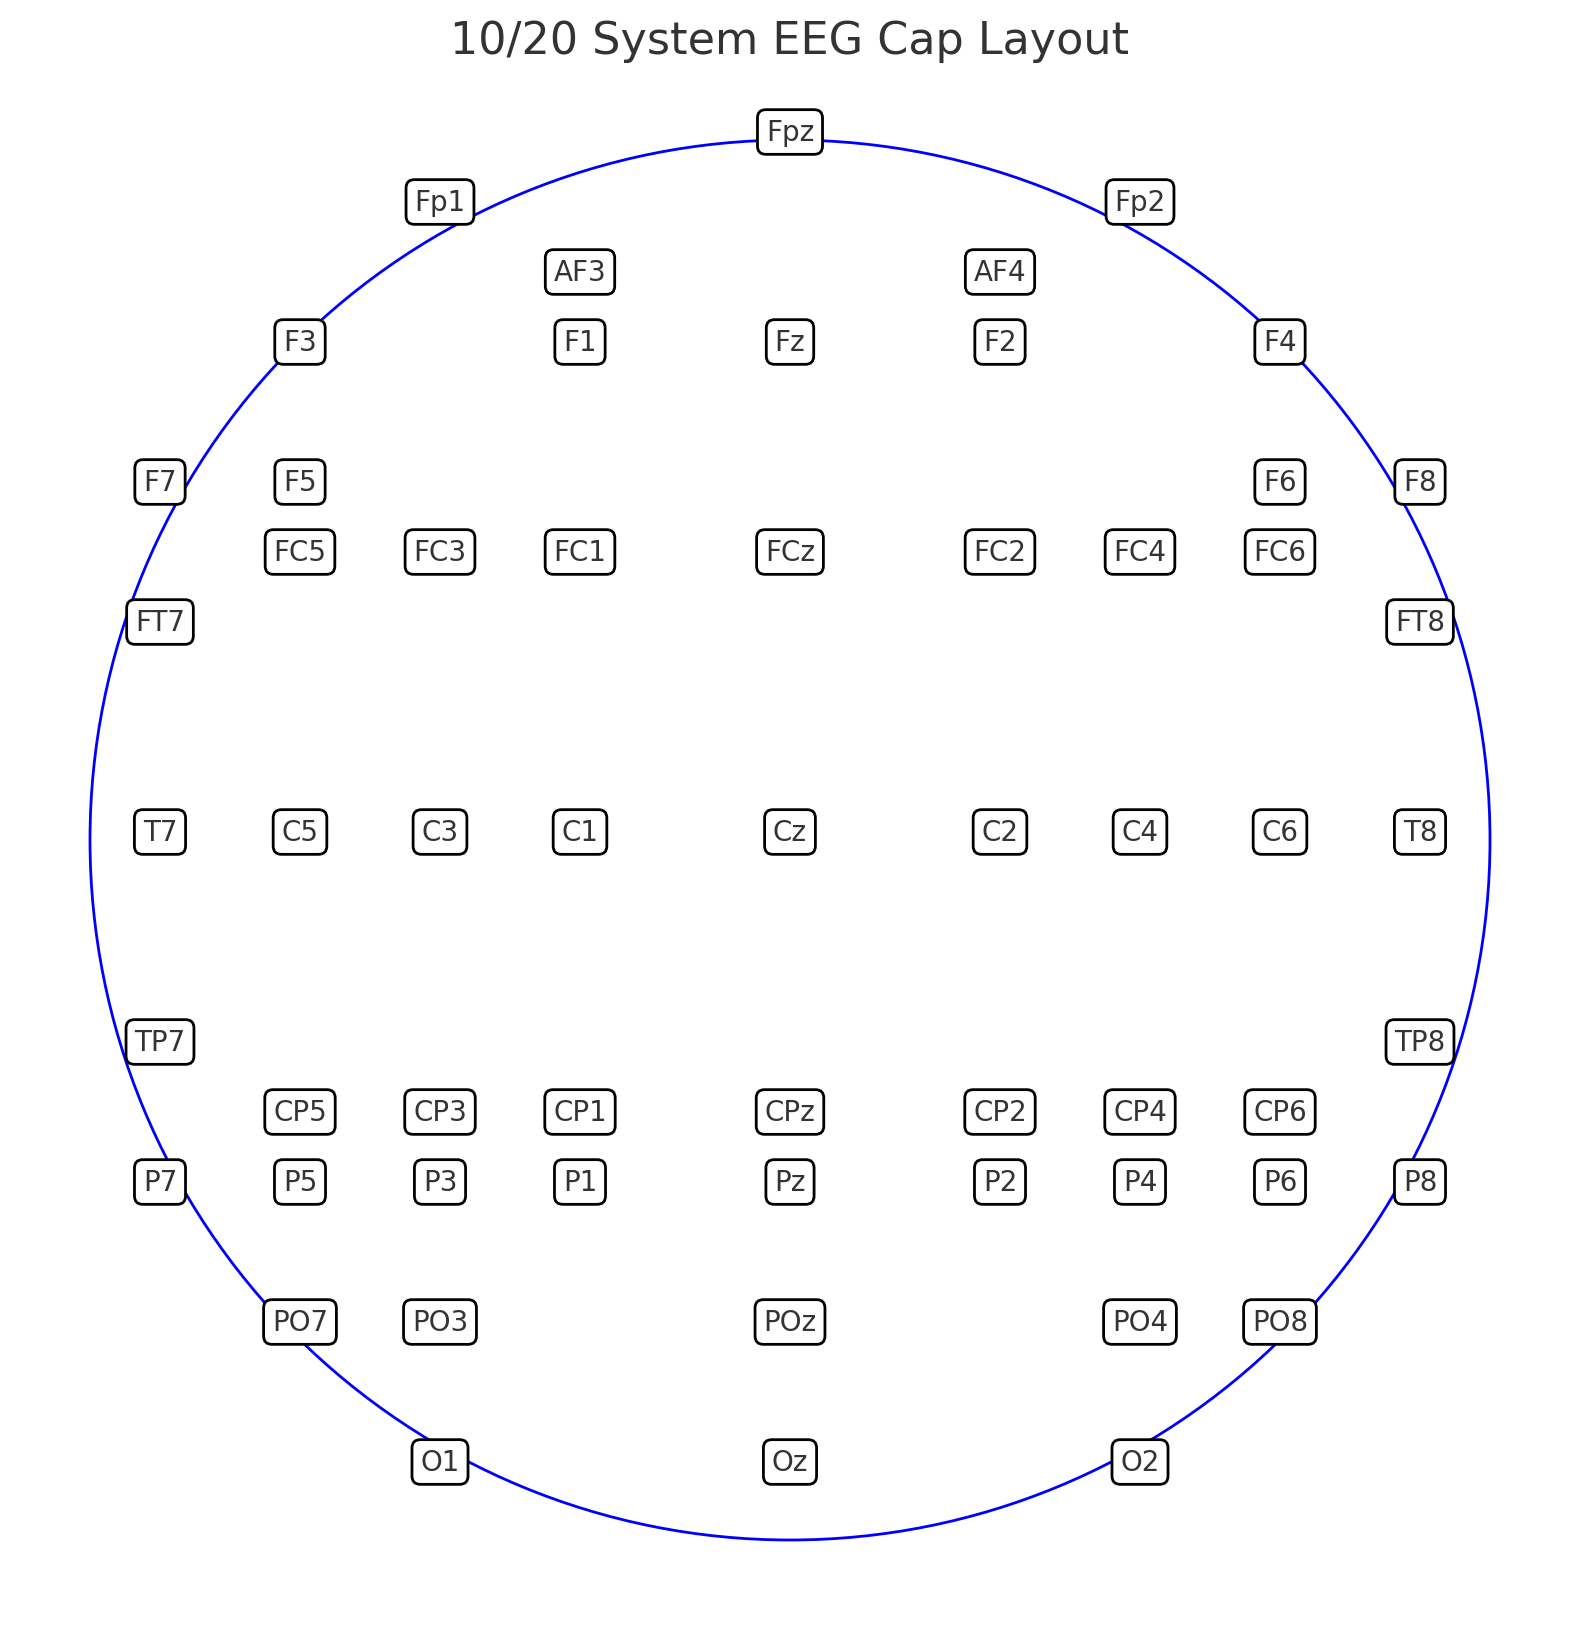
\includegraphics[width=0.5\textwidth]{Figures/Methodology/thesis_eeg_cap}
    \caption{Position of the selected EEG Channels using the reference 10/20 system.}
    \label{fig:eeg_channels}
\end{figure}

\section{Data Augmentation}
Data augmentation is a technique used to increase the size of the training dataset.
It is used to improve the performance of the machine learning model and to generate new data points by applying transformations to the existing ones.
Data augmentation is used to test the generalization of the machine learning model, thus reduce overfitting.
In this project, we applied multiple data augmentation techniques, such as random sampling of the data points, stochastic noise addition, and generation of new data points using GANs.
After testing the quality of the generated data, we found out that the best results were obtained by the noise addition technique and the GAN.

\subsection*{Parameters Used}
For each class, we created a separate genereator, which was used to generate the data points.
Since we are using 4 classes, we created 4 generators using the noise injection and 4 generators using the GAN.
\paragraph*{Stochastic Noise Injection}
The noise injection generator was created by taking the third and fourth quartile of the data points to reduce the size.
After this, we randomly selected a data point from the reduced dataset and added a Gausian noise to it.
The noise was generated using the ``numpy.random.normal'' function, with a mean of 0 and a standard deviation of 1.
As parameter we also provided the shape of the data point, which was used to generate the noise in the correct format.
\paragraph*{Generative Adversarial Networks}
The GAN generator was composed of two networks: the generator~(EEGFuseNet) and the discriminator~(EFDiscriminator), both network were taken from the models provided by the library ``torcheeg''~\cite{zhang2024torcheeg}.
These models have been reimplemented in torcheeg following their description from~\cite{liang2021eegfusenet} and their architecture is presented in Figure~\ref{fig:gan_paper}.
\begin{figure}[!htbp]
    \centering
    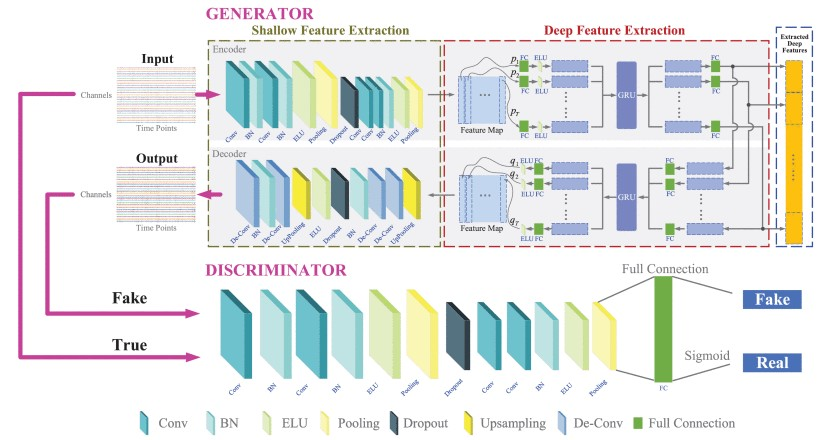
\includegraphics[width=\textwidth]{Figures/Methodology/GAN}
    \caption{Architecture of the GAN model. 
    We can notice the architecture of the Generator that studies the EEG input, extracts features from it, and then uses these information to generate new datapoints. 
    The Figure also presents the architecture of the Discriminator that receives an EEG signal, and has to decide if it is real or fake. Image from~\cite{liang2021eegfusenet}}\label{fig:gan_paper}
\end{figure}


As for the training parameters, we used the following:
\begin{itemize}
    \item \textbf{Loss Function}: Binary Cross Entropy
    \item \textbf{Optimizer}: Adam
    \item \textbf{Learning Rate}: 0.0002
    \item \textbf{Train Epochs}: 100 epochs, each epoch changing the number of steps for generator and discriminator.
\end{itemize}
\paragraph*{Train Epochs}
As visible in Listing \ref{code:gan_train_snippet}, the training of the GAN was divided into two parts, the generator and the discriminator.
The full training lasted 100 epochs.
During each epoch, we trained the generator and the discriminator for a different number of steps.
The discriminator was trained first, starting with 1000 steps, and decreasing each epoch until 10 steps.
The generator was trained after the discriminator, starting with 10 steps, and increasing each epoch until 1000 steps.
\lstinputlisting[language=python, caption={GAN Train Loop Snippet}, label={code:gan_train_snippet}, captionpos=b]{Code/train_gan.py}

\section{Classification Model}
The classification model is a machine learning or deep learning model used to classify the data points.
It is used to predict the class or label to which the input data point belongs.
In this project, we decided to train a set of machine learning and deep learning models to classify the data points.
Some of these methods, including support vector machines, linear discriminant analysis and convolutional neural networks, have been used as baseline models, the proposed LSTM (Figure~\ref{fig:lstm_model}) and Attention-based (Figure~\ref{fig:attention_model}) methods have been used as the main models.
The models were trained using the available datasets, and validated using the test set.
Also, the models where evaluated using the generated data points to test their generalization capabilities.
It is important to notice, that the main difference in the models, a part from the architecture, and the number of parameters, is the difference in how they understand the temporal dependencies of the EEG signal.
The LSTM model uses the recurrent layers to understand how each timepoint in the signal is related to the others, while the Attention model uses the attention mechanism to understand the signal in a more global way.

\subsection*{Parameters Used}
The neural network models were trained using the following parameters:
\begin{itemize}
    \item \textbf{Loss Function}: Categorical Cross Entropy
    \item \textbf{Optimizer}: Adam
    \item \textbf{Learning Rate}: 0.01
    \item \textbf{Train Epochs}: 1000 epochs
    \item \textbf{Metrics}: Accuracy and Confusion Matrix
\end{itemize}
While the machine learning models only used the default parameters provided by the library and were trained for 1000 epochs.
\begin{figure}[!htbp]
    \centering
        \centering    
        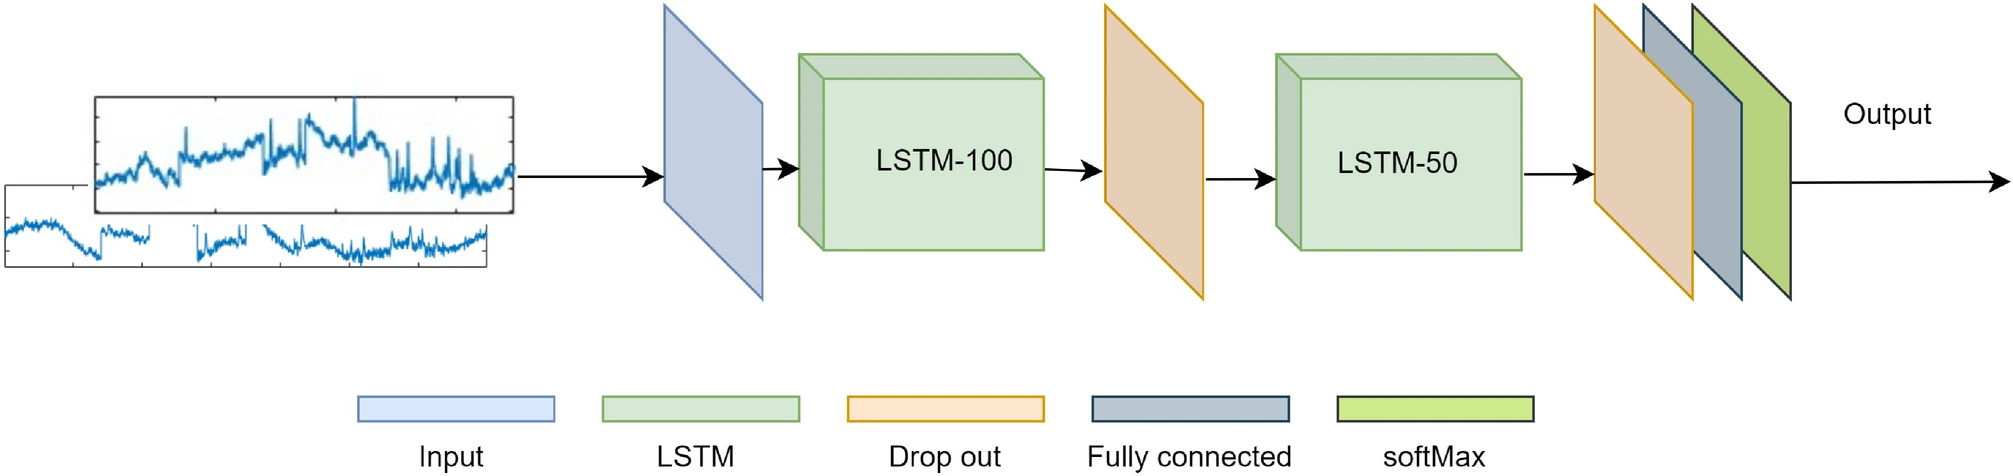
\includegraphics[width=\textwidth]{Figures/Methodology/LSTM}
        \caption{Architecture of the LSTM-based model.
        The EEG Signal passes by the LSTM layers, that are able to understand the temporal dependencies of the signal, and then the output is passed to the Dense layer that classifies it in one of the provided classes.
        Image from~\cite{sharma_deep_2023}}\label{fig:lstm_model}
\end{figure}
\begin{figure}[!htbp]
        \centering
        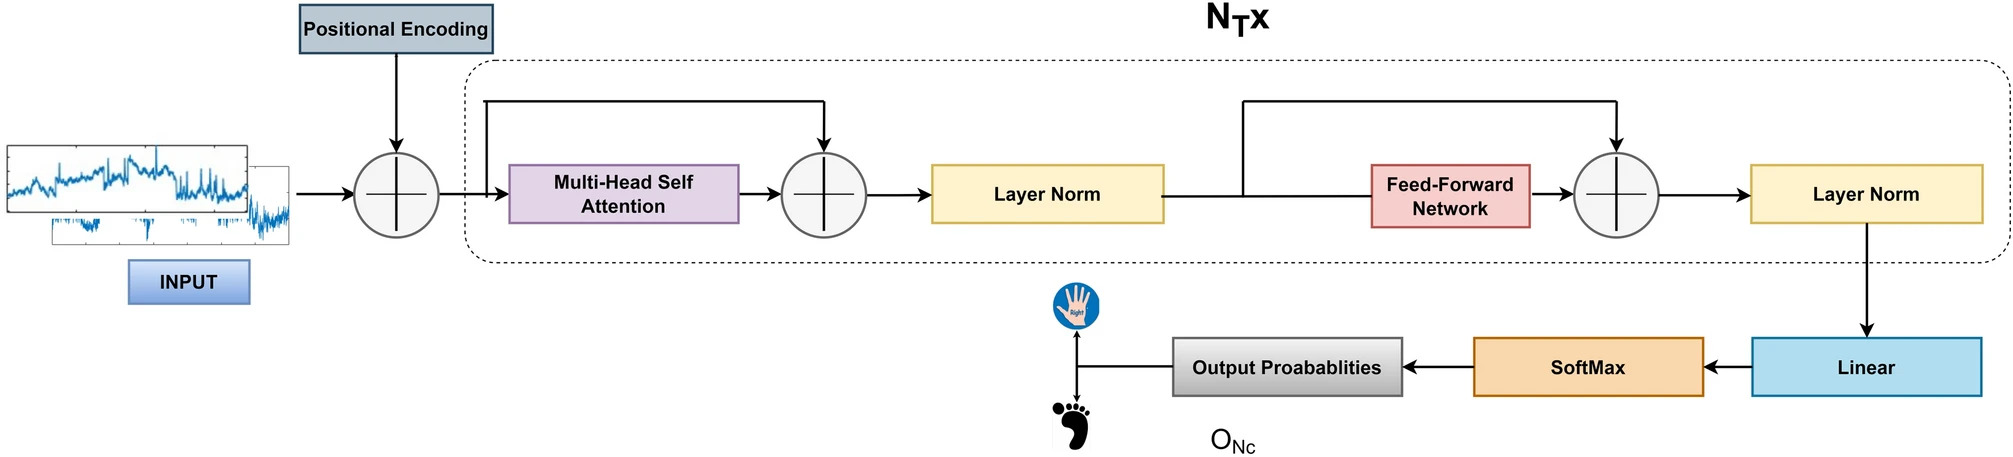
\includegraphics[width=\textwidth]{Figures/Methodology/Attention}
        \caption{Architecture of the Transformer-based model. 
        The EEG Signal is positional encoded and then passed to four consecutive Attention layers, that are understand the temporal dependencies of the signal, and then the output is passed to the Dense layer that classifies it in one of the provided classes.
        Image from~\cite{sharma_deep_2023}}\label{fig:attention_model}
\end{figure}

\section{Virtual Environment}
The virtual environment is a computer-generated environment that simulates the real world or a specific scenario.
It is used to test the performance and usability of the machine learning model, and to evaluate the user experience.
In this project, we developed two virtual environments: an infinite runner game where the user can jump over obstacles or move to left or right, and a maze where the user can freely move their character to collect coins.
The virtual environments were developed using the Unity game engine, version 2022.3.20f1, and were designed to be simple and easy to use, and to provide a fun and engaging experience for the user.
The virtual environments were also designed to be controller agnostic, requiring a WebSocket connection to receive the character input commands.
\subsection*{Unity Packages and Assets Used}
% The main packages used are:
% \begin{itemize}
%     \item TextMeshPro\footnote{Documentation available at the following link: \url{https://docs.unity3d.com/Manual/com.unity.textmeshpro.html}}: for the Main Menu and the in-game information.
%     \item Starter Assets \textemdash Third Person Controller\footnote{Removed from Unity Asset Store}: for the player avatar and main movement logic and animations.
%     \item Native Websocket\footnote{Open source package for Unity, available at the following link: \url{https://github.com/endel/NativeWebSocket}}: to receive the character control commands from the framework.
%     \item AI Navigation\footnote{Documentation available at the following link: \url{https://docs.unity3d.com/Packages/com.unity.ai.navigation@2.0/manual/index.html}}: to move the character in the Maze game.
%     \item Maze Generator\footnote{Asset available at the following link: \url{https://assetstore.unity.com/packages/tools/modeling/maze-generator-38689}}: to generate the maze in the Maze game.
% \end{itemize}
% \todo{make text instead of bullet list}
The main packages used are TextMeshPro\footnote{Documentation available at the following link: \url{https://docs.unity3d.com/Manual/com.unity.textmeshpro.html}}, for the Main Menu and the in-game information, Starter Assets \textemdash Third Person Controller, for the player avatar and main movement logic and animations, Native Websocket\footnote{Open source package for Unity, available at the following link: \url{https://github.com/endel/NativeWebSocket}}, to receive the character control commands from the framework, AI Navigation\footnote{Documentation available at the following link: \url{https://docs.unity3d.com/Packages/com.unity.ai.navigation@2.0/manual/index.html}}, to move the character in the Maze game, and Maze Generator\footnote{Asset available at the following link: \url{https://assetstore.unity.com/packages/tools/modeling/maze-generator-38689}}, to generate the maze in the Maze game.


\subsection*{Infinite Runner Game}
The infinite runner game (Figure~\ref{fig:infinite_runner}) was developed to test the performance of the machine learning model in a fast-paced environment.
The game is a simple 3D game where the player can jump over obstacles or move to turn to the left or right on crossroads.
The player character moves forward automatically and the speed is controlled by a sigmoid-like curve.
The user can provide the direction commands by thinking about the desired movement.
The path and the obstacles are generated randomly and the game logic was implemented from scratch.
The path is a modular prefab, showed in the previous chapter (Chapter~\ref{ch:approach}), only the first two tiles are manually specified, the rest is generated randomly.
Techniques to delete the parts that are not visible and to generate new parts are used to keep the game running smoothly.
Also, the obstacles are generated randomly, with a fixed probability of appearing.
The code is modular, with the main logic separated from the Unity components.
This allows for easy modification and extension of the game, for easy integration of new obstacles or changes in the path.
After some tests, we decided to exclude the Infinite Runner game from the final evaluation, as the game was too fast and while the user was able to provide the commands in time using the keyboard, the actual EEG signals required more time to be processed, resulting in a poor user experience. 

In Figure~\ref{fig:infinite_runner_path_generation} we can see the algorithm used to generate the path in the Infinite Runner game.
The actual algorithm is event based, therefore providing a code snippet is not simple and will not make the logic easy to understand.
The algorithm is divided into multiple steps, as the player autonomously moves, the path is generated in front of it.
At the end of each path tile, the user automatically crosses a collider that triggers the generation of the next tile.
If the player crosses a collider that is part of a crossroad, the player is rotated along with the camera to face the new direction.
After this eventual rotation, the not visible tiles are deleted, and the algorithm starts generating the new tiles.
The algorithm randomly decides if the new tile has a left, right and/or forward tile at the end.
To avoid the game from automatically ending, there will always be at least one tile.
For each of the possible tiles, up to three, that has to be generated, the algorithm randomly decides if the tile has an obstacle, and in case, generates it.
After generating the new tiles, the algorithm removes the walls to allow continuous movement between the tiles and completes its execution.
In the diagram it loops back to the first step, as the player keeps moving forward during this whole process and the algorithm has to generate the next tiles.
In figure we can notice the ``Generate New Tiles'' step is dashed, this is because it has to be considered as a comment, describing the next steps, and not as a real step in the algorithm.

\begin{figure}[!htbp]
    \centering
    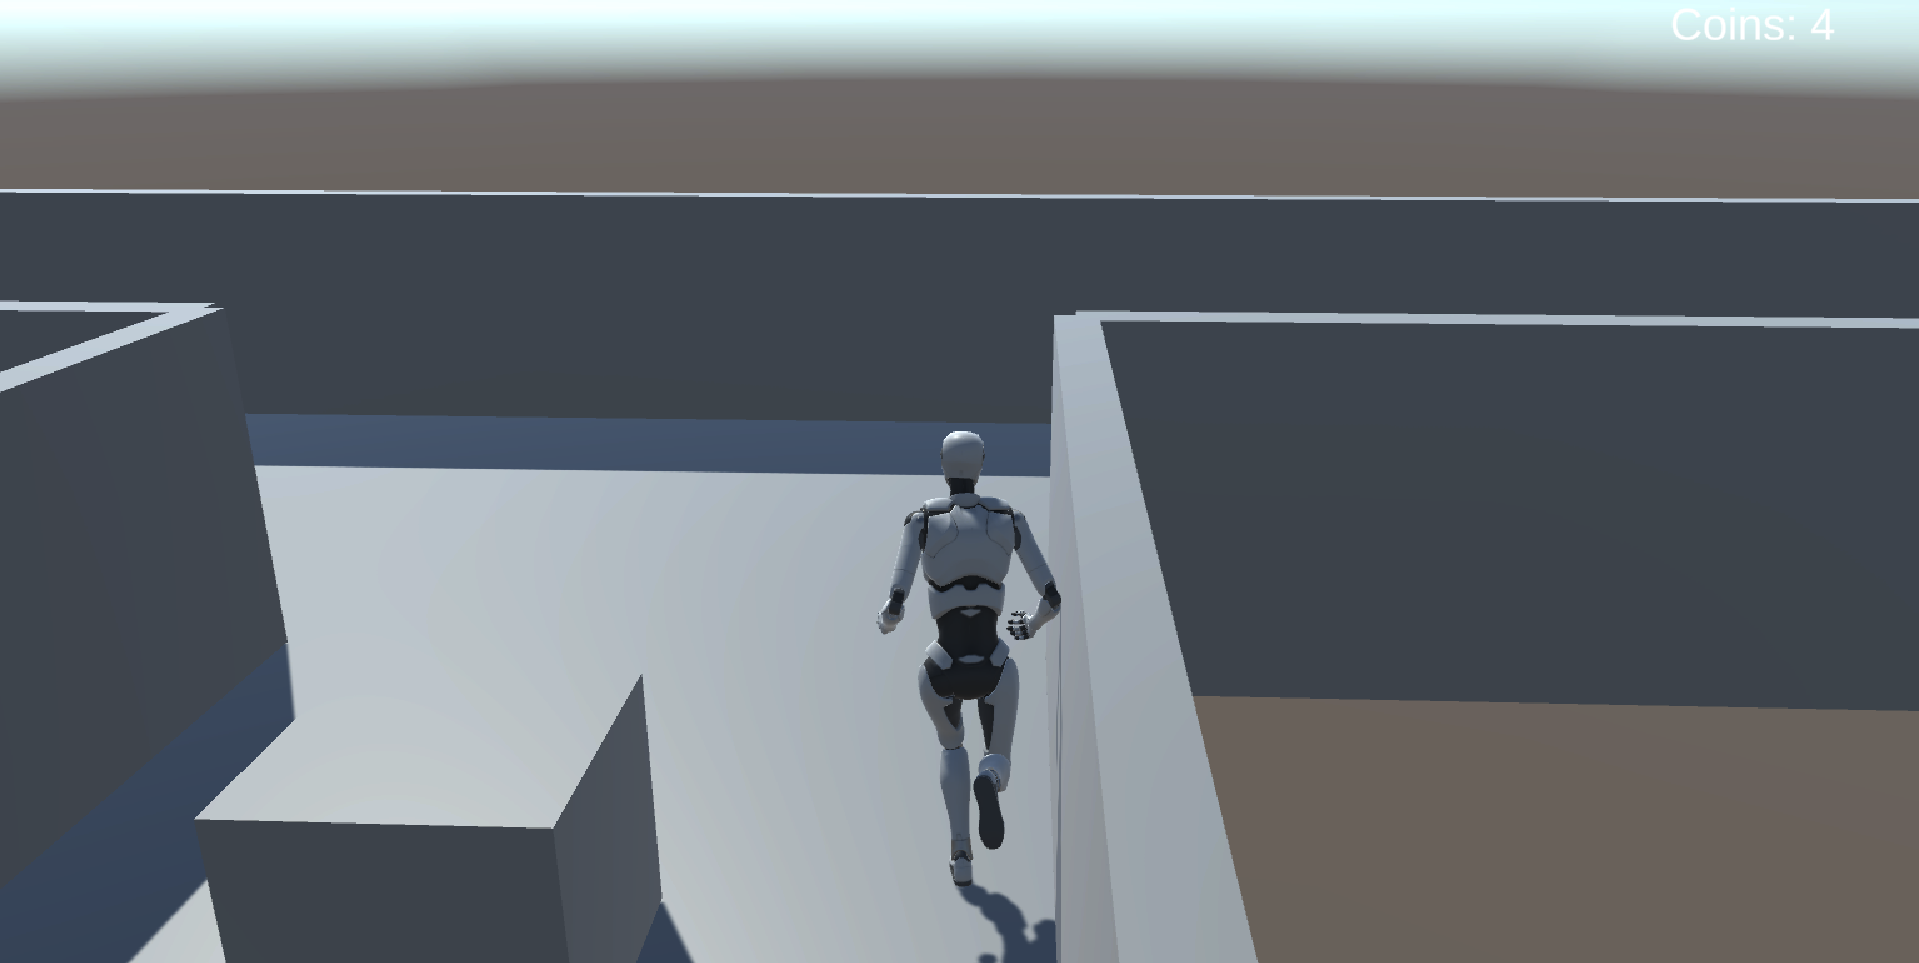
\includegraphics[width=0.8\textwidth]{Figures/Methodology/infinite_runner}
    \caption{Infinite Runner Virtual Environment. We can notice the player automatically moving forward, an obstacle on its left and the crossroad in front of it.}\label{fig:infinite_runner}
\end{figure}
\begin{figure}[!htbp]
    \centering
    % Flowchart representing code logic:
    % 1. Player walks in the path
    % 2. Delete not visible tiles
    % 3. Start generate new tiles
    % 3.a Has this tile a left tile at the end
    % 3.b Has this tile a right tile at the end
    % 3.c Has this tile a forward tile at the end
    % 4. Foreach next tile at the end
    % 4.a Has next tile a obstacle
    % 4.a.yes Generate obstacle for tile
    % 4.a.no Continue
    % 4.b Delete wall correspondig to next tile
    % 5. Tile generated
    % Loop back to 1
    \scalebox{0.4}{
    \begin{tikzpicture}[
        squarednode/.style={rectangle, draw=black, very thick, minimum size=5mm},
        diamondnode/.style={diamond, draw=black, very thick},
        ]
        %Nodes
        \node[squarednode] (player) {Player Walks};
        \node[squarednode, below=of player] (rotate) {Eventually Rotate Player and Camera};
        \node[squarednode, below=of rotate] (delete) {Delete Not Visible Tiles};
        \node[squarednode, below=of delete, dashed] (generate) {Generate New Tiles};
        \node[diamondnode, below=of generate] (hasleft) {Has Left Tile};
        \node[squarednode, below right=of hasleft] (generateleft) {Generate Left Tile};
        \node[diamondnode, below=of hasleft] (hasright) {Has Right Tile};
        \node[squarednode, below right=of hasright] (generateright) {Generate Right Tile};
        \node[diamondnode, below=of hasright] (hasforward) {Has Forward Tile};
        \node[squarednode, below right=of hasforward] (generateforward) {Generate Forward Tile};
        \node[squarednode, below=of hasforward] (foreach) {Foreach Next Tile};
        \node[diamondnode, below=of foreach] (hasobstacle) {Has Obstacle};
        \node[squarednode, below right=of hasobstacle] (generateobstacle) {Generate Obstacle};
        \node[squarednode, below=of hasobstacle] (deletewall) {Delete Wall};
        \node[squarednode, below=of deletewall] (tilegenerated) {Tile Generated};
        %Lines
        \draw[->] (player) -- node[right] {Cross end of path collider} (rotate);
        \draw[->] (rotate) -- (delete);
        \draw[->] (delete) -- (generate);
        \draw[->] (generate) -- (hasleft);
        \draw[->] (hasleft) -- node[right] {No} (hasright);
        \draw[->] (hasleft) -- node[right] {Yes} (generateleft);
        \draw[->] (generateleft) -- (hasright);
        \draw[->] (hasright) -- node[right] {No} (hasforward);
        \draw[->] (hasright) -- node[right] {Yes} (generateright);
        \draw[->] (generateright) -- (hasforward);
        \draw[->] (hasforward) -- node[right] {No} (foreach);
        \draw[->] (hasforward) -- node[right] {Yes} (generateforward);
        \draw[->] (generateforward) -- (foreach);
        \draw[->] (foreach) -- (hasobstacle);
        \draw[->] (hasobstacle) -- node[right] {Yes} (generateobstacle);
        \draw[->] (hasobstacle) -- node[right] {No} (deletewall);
        \draw[->] (deletewall) -- (tilegenerated);
        \draw[->] (generateobstacle) -- (deletewall);
        \draw[->] (tilegenerated) to[out=180, in=180] (foreach);
    \end{tikzpicture}
    }
    \caption{Infinite Runner Path Generation Algorithm}\label{fig:infinite_runner_path_generation}
\end{figure}

\subsection*{Maze Game}
The Maze Walker~\ref{fig:maze} game was developed to test the performance of the machine learning model in a more complex environment.
The game is a 3D walking game where the player can move freely in a maze to collect coins.
The maze is generated randomly using the Maze Generator package.
The player character can freely move around thanks to the integration of the AI Navigation package.
As the movement is autonomous, the role of the user is to provide the direction commands by thinking about the desired movement, left, right or forward.
Upon collecting all coins, the user proceeds to the next level, where the maze is regenerated and the coins are placed in different, randomly selected positions.

\begin{figure}[!htbp]
    \centering
    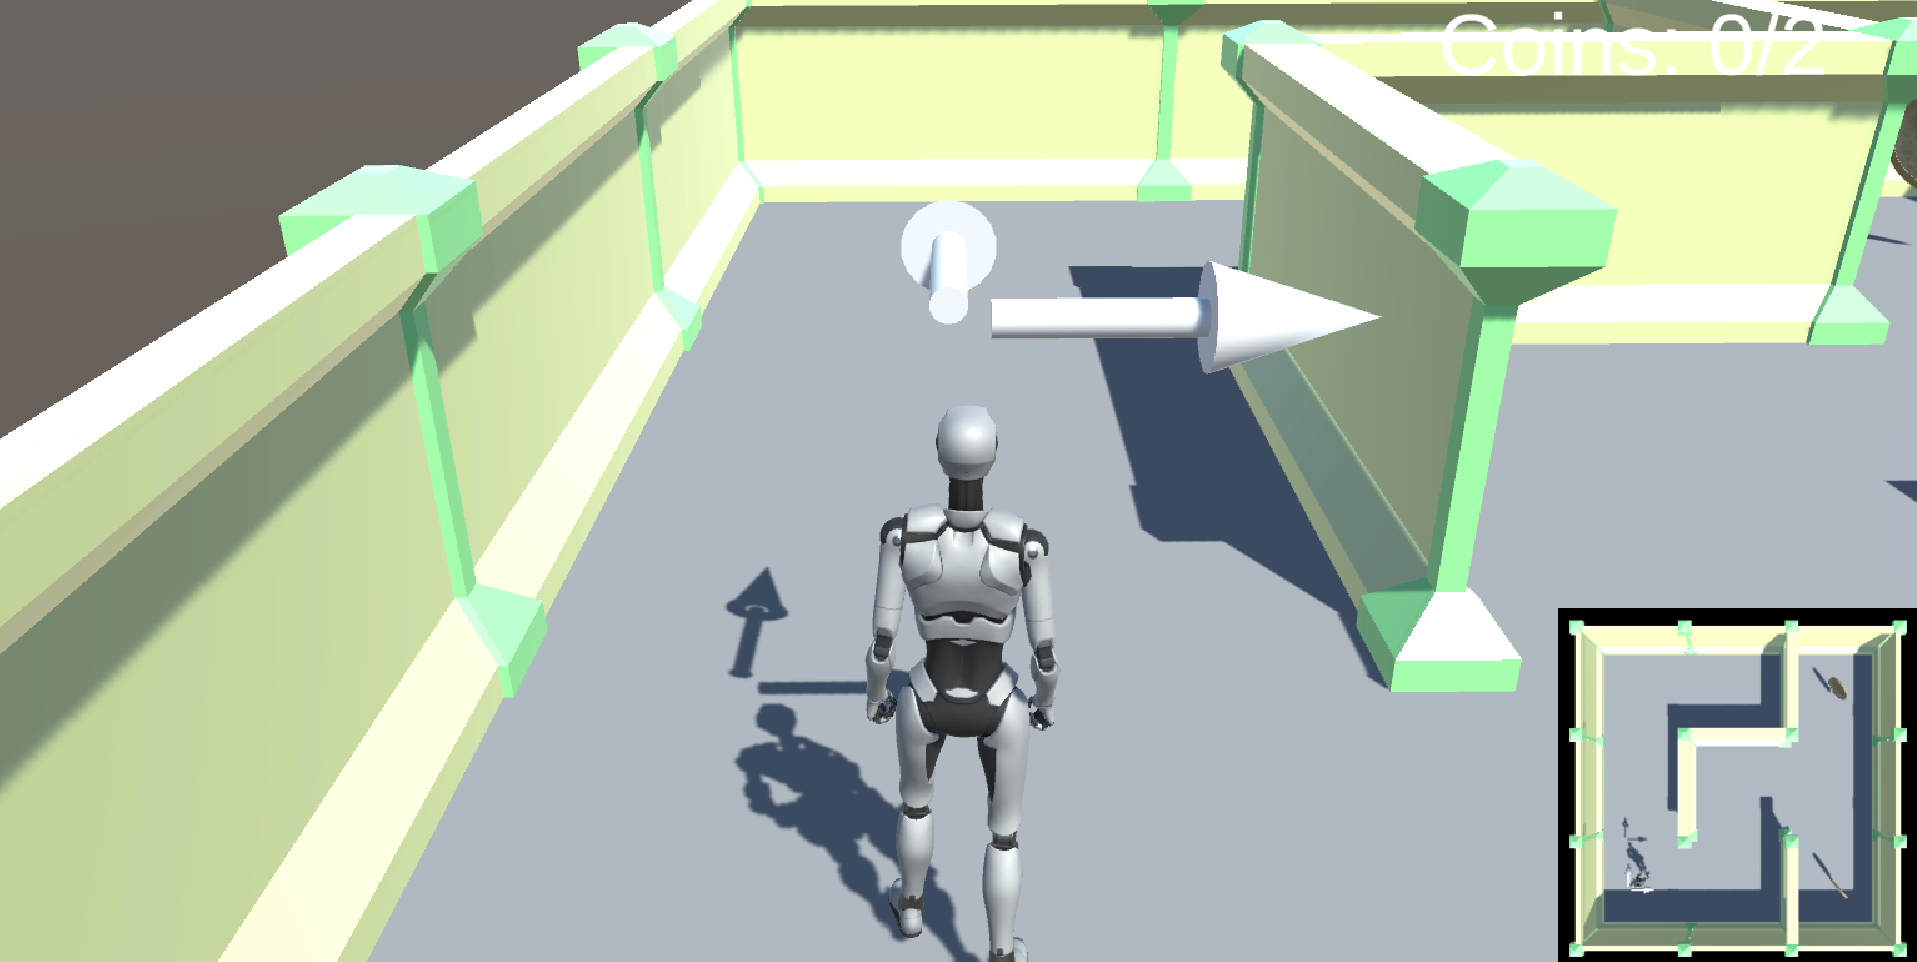
\includegraphics[width=0.8\textwidth]{Figures/Methodology/maze}
    \caption{Maze Virtual Environment. We can notice the player in the maze, with the minimap on the bottom right corner, and the coins to collect, also, the arrows on top of the avatar are used to indicate the available movement directions.}\label{fig:maze}
\end{figure}